\section{Model\-Car\-Smooth  Class Reference}
\label{classModelCarSmooth}\index{ModelCarSmooth@{Model\-Car\-Smooth}}
The same model as {\bf Model2DRigid\-Car\-Smooth} {\rm (p.\,\pageref{classModel2DRigidCarSmooth})}. 


{\tt \#include $<$modelcar.h$>$}

Inheritance diagram for Model\-Car\-Smooth::\begin{figure}[H]
\begin{center}
\leavevmode
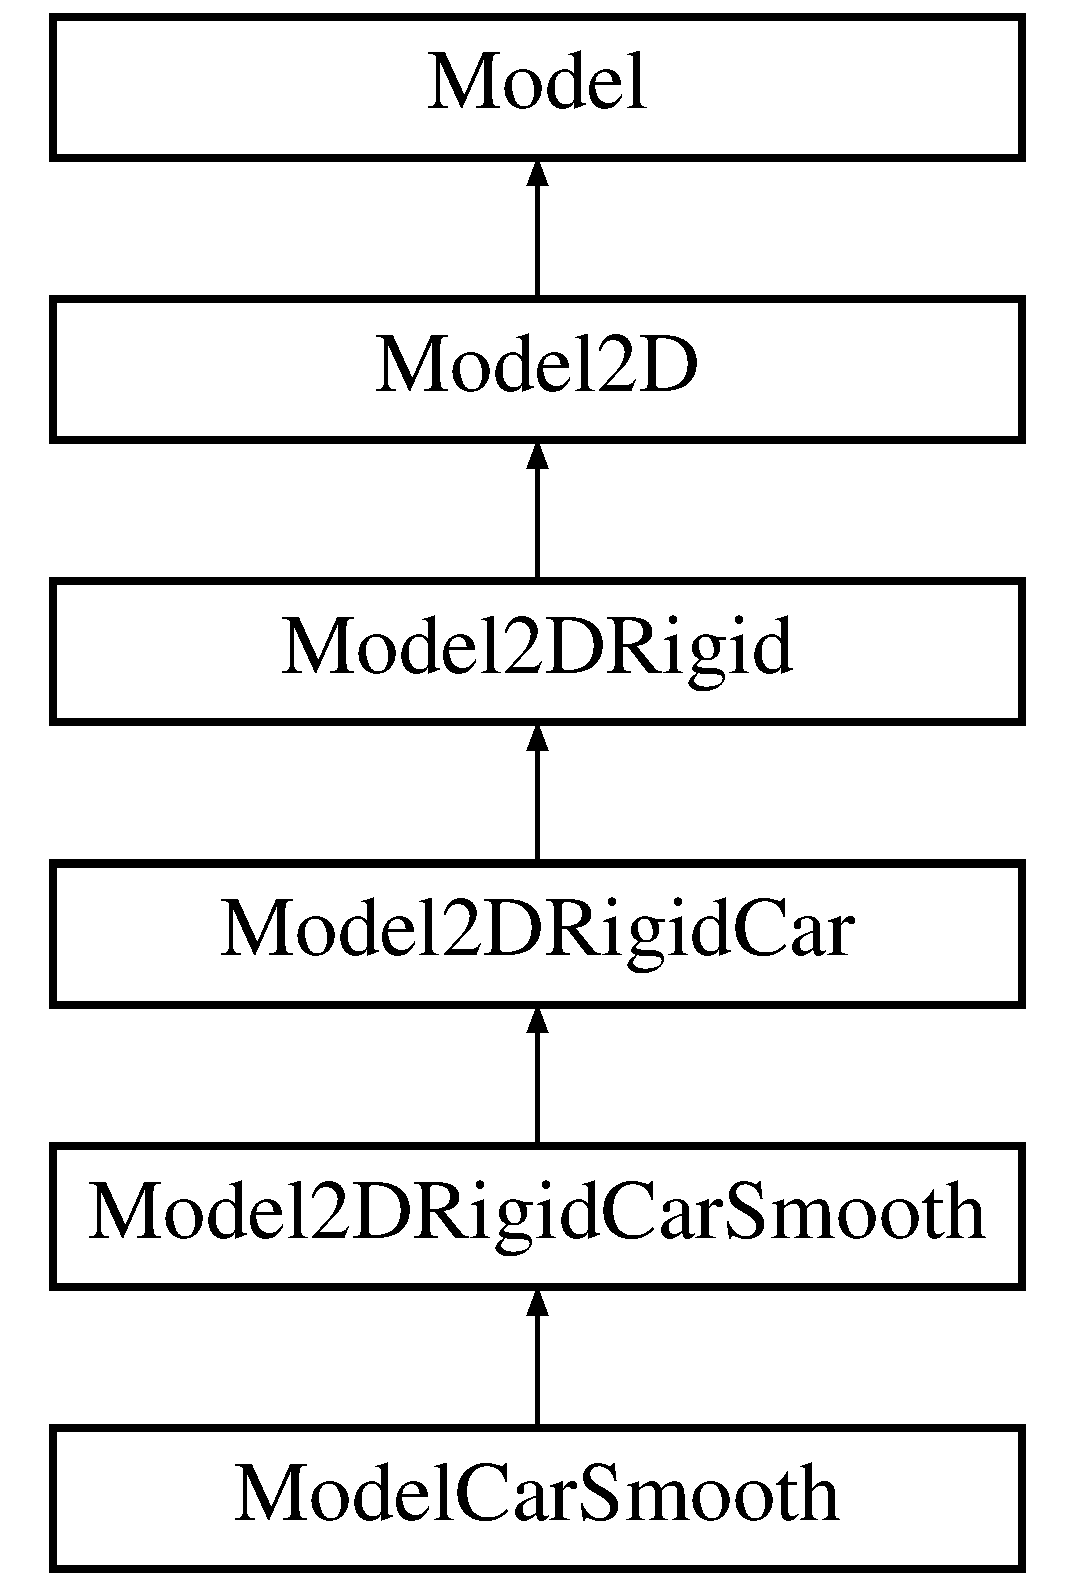
\includegraphics[height=6cm]{classModelCarSmooth}
\end{center}
\end{figure}
\subsection*{Public Methods}
\begin{CompactItemize}
\item 
{\bf Model\-Car\-Smooth} (string path)
\item 
virtual {\bf $\sim$Model\-Car\-Smooth} ()
\item 
virtual {\bf MSLVector} {\bf State\-To\-Configuration} (const {\bf MSLVector} \&{\bf x})
\begin{CompactList}\small\item\em A method that converts a {\bf Model} {\rm (p.\,\pageref{classModel})} state in to a {\bf Geom} {\rm (p.\,\pageref{classGeom})} configuration.\item\end{CompactList}\end{CompactItemize}


\subsection{Detailed Description}
The same model as {\bf Model2DRigid\-Car\-Smooth} {\rm (p.\,\pageref{classModel2DRigidCarSmooth})}.



\subsection{Constructor \& Destructor Documentation}
\index{ModelCarSmooth@{Model\-Car\-Smooth}!ModelCarSmooth@{ModelCarSmooth}}
\index{ModelCarSmooth@{ModelCarSmooth}!ModelCarSmooth@{Model\-Car\-Smooth}}
\subsubsection{\setlength{\rightskip}{0pt plus 5cm}Model\-Car\-Smooth::Model\-Car\-Smooth (string {\em path})}\label{classModelCarSmooth_a0}


\index{ModelCarSmooth@{Model\-Car\-Smooth}!~ModelCarSmooth@{$\sim$ModelCarSmooth}}
\index{~ModelCarSmooth@{$\sim$ModelCarSmooth}!ModelCarSmooth@{Model\-Car\-Smooth}}
\subsubsection{\setlength{\rightskip}{0pt plus 5cm}virtual Model\-Car\-Smooth::$\sim$Model\-Car\-Smooth ()\hspace{0.3cm}{\tt  [inline, virtual]}}\label{classModelCarSmooth_a1}




\subsection{Member Function Documentation}
\index{ModelCarSmooth@{Model\-Car\-Smooth}!StateToConfiguration@{StateToConfiguration}}
\index{StateToConfiguration@{StateToConfiguration}!ModelCarSmooth@{Model\-Car\-Smooth}}
\subsubsection{\setlength{\rightskip}{0pt plus 5cm}{\bf MSLVector} Model\-Car\-Smooth::State\-To\-Configuration (const {\bf MSLVector} \& {\em x})\hspace{0.3cm}{\tt  [virtual]}}\label{classModelCarSmooth_a2}


A method that converts a {\bf Model} {\rm (p.\,\pageref{classModel})} state in to a {\bf Geom} {\rm (p.\,\pageref{classGeom})} configuration.



Reimplemented from {\bf Model2DRigid\-Car\-Smooth} {\rm (p.\,\pageref{classModel2DRigidCarSmooth_a4})}.

The documentation for this class was generated from the following files:\begin{CompactItemize}
\item 
{\bf modelcar.h}\item 
{\bf modelcar.C}\end{CompactItemize}
